\chapter{Grundlagen}
\label{chapter_Grundlagen}

Bei der Entwicklung des Teststandes kommen verschiedene Systeme und Konzepte zum Einsatz. Dieses Kapitel befasst sich mit der C++ Klassenbibliothek Qt und der Frage, was ist die Degradation oder ein Embedded-Linux-System. Des Weiteren wird auf das Konzept einer Datenbank und der Evaluierung der beiden Datenbanksysteme MySQL und SQLite eingegangen.

\section{Degradation}
\label{section_Degradation}
Der Hauptgrund für mechanisches Versagen im Lebenszyklus eines Systems oder Bauelementes, liegt an der langsamen Ansammlung von nicht reversiblen Schäden. Dieser Prozess ist bekannt als Degradation (vgl. \cite{zhou2011}).\\
Die Schwierigkeit liegt in der Feststellung des mechanischen Versagens in messbaren Schritten.\\
So ist die Bestimmung der Lebenszeit über die Zeit bis zum Ausfall zeitaufwändig. Einfacher ist es die Leistung des Bauelementes oder Systems zu erfassen, z.B. die optische Leistung einer \ac{LED}. Auf diesem Weg kann ein Trend ausgemacht werden.\\
Um die Länge des Lebenszyklus eines Bauelementes bestimmen zu können, wird die Leistung dessen unter Last über einen langen Zeitraum hinweg aufgezeichnet. Anhand der daraus resultierenden Daten kann die zu erwartende Länge des Lebenszyklus ermittelt werden.\\
In Abbildung \ref{figure_Degradation} ist ein Beispiel für erfasste Daten zu sehen. Sie zeigt die relative Abweichung der optischen Leistung über die Zeit von sieben verschiedenen \acp{LED}. 

 
\begin{figure}[H]
\begin{center}
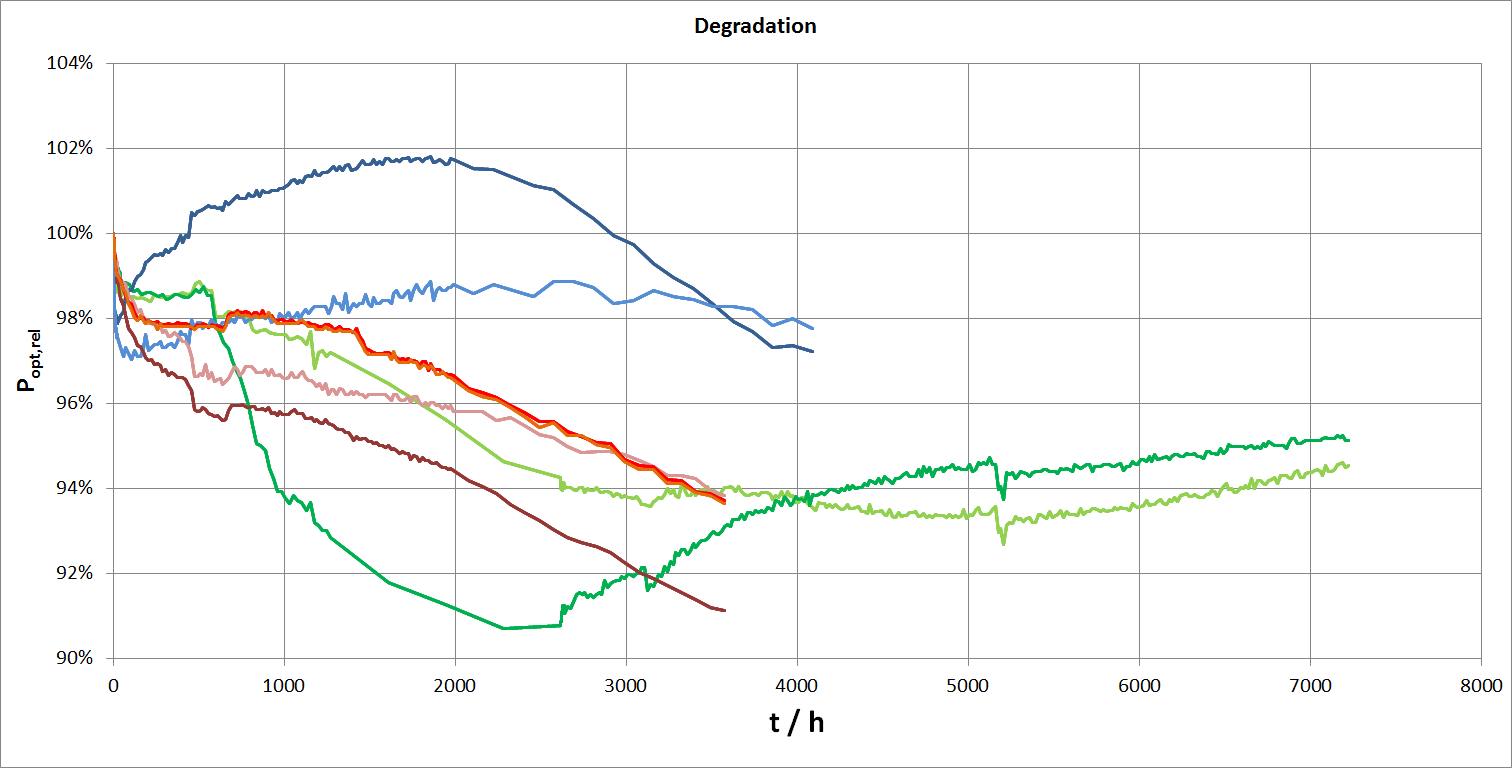
\includegraphics[width=0.8\textwidth]{img/general/Degradation.png}
\caption{Aufgezeichnete Degradation}
\label{figure_Degradation}
\end{center}
\end{figure}



\section{Qt}
\label{section_Qt}
Qt \cite{qtproject} ist eine umfangreiche C++-Klassenbibliothek zur Gestaltung und Entwicklung von Anwendungen. Vor allem bei Applikationen mit grafischen Benutzeroberflächen (englisch: \ac{GUI}) ist Qt sehr beliebt. \\
Zusätzlich bringt Qt eine große Auswahl an Tools und Modulen mit sich, welche die Programmierung erheblich erleichtern (z.B. Netzwerkprogrammierung, Datenbankanbindung, OpenGL, etc.). \\
Ein weiterer Vorteil ist die Plattformunabhängigkeit. So unterstützt Qt aktuell (Version 5.4, 10. Dezember 2014) einen Großteil der aktuellen Betriebssysteme wie Windows, Linux, Android, iOS und einige mehr. Die hohe Kompatibilität wird dadurch gegeben, dass Qt die meisten Systemaufrufe abstrahiert.

\subsection{Signale und Slots}
\label{QtSignaleSlots}
Die Kommunikation unter den Objekten in Qt erfolgt über Signale und Slots. Dabei sendet ein Objekt ein Signal aus und ein anderes empfängt dieses. Dafür muss zunächst eine Verbindung zwischen den Objekten aufgebaut werden. Das erfolgt mit dem \textit{connect}-Statement.\\

\begin{lstlisting}[caption={Qt \textit{connect}-Statement},label=lst_QtConnect]
connect(Calculate, SIGNAL(clicked()), this, SLOT(addAB()));
\end{lstlisting}

Im Quellcode \ref{lst_QtConnect} wird ein Beispiel für die Verbindung von zwei Objekten mit dem \textit{connect}-Statement gezeigt. Hier wird das Signal \textit{clicked()} des Objektes \textit{Calculate} mit dem Slot \textit{addAB()} des Objektes \textit{this}, was dem aktuellen Objekt entspricht, verbunden. \\

\begin{lstlisting}[caption={Qt \textit{emit}-Statement},label=lst_QtEmit]
void Calculate::my_function(){
	/*
	Do Something
	*/
	emit clicked();	
}
\end{lstlisting}

Im Quellcode \ref{lst_QtEmit} wird das Signal \textit{clicked()} mittels \textit{emit}-Statement ausgelöst und der Slot des verbundenen Objektes aktiviert. Somit ist es möglich beispielsweise die GUI und den Hauptprogrammablauf von einander zu trennen und lediglich über Signale und Slots kommunizieren zu lassen. Dadurch agieren beide Teile komplett unabhängig von einander.

\subsection{Entwicklungsumgebung}
Als Entwicklungsumgebung (englisch: \ac{IDE}) dient der Qt Creator (siehe Abbildung \ref{QtCreator}), welcher Teil des \ac{SDK} von Qt ist und sowohl auf Linux, Windows als auch Mac OS X zur Verfügung steht. Er kommt mit einem Debugger, einem integrierten \ac{GUI} Designer und einem Texteditor mit Funktionen wie Syntax-Hervorhebung und automatischer Vervollständigung. \\
Dabei kommen gängige Compiler wie MinGW unter Windows zum Einsatz und es besteht die Möglichkeit eigene Toolchains anzulegen. \\
Eine Toolchain dient zum Übersetzen von Quellcode auf einem Host-System für ein Ziel-System. Sie setzt sich meistens aus einer Kette von Werkzeugen zusammen, welche nacheinander für die Übersetzung des Quellcodes sorgen. Somit ist es möglich, einen Programmcode auf einem Windowsrechner zu schreiben und anschließend für ein Linux-System zu übersetzen.

\begin{figure}[H]
\begin{center}
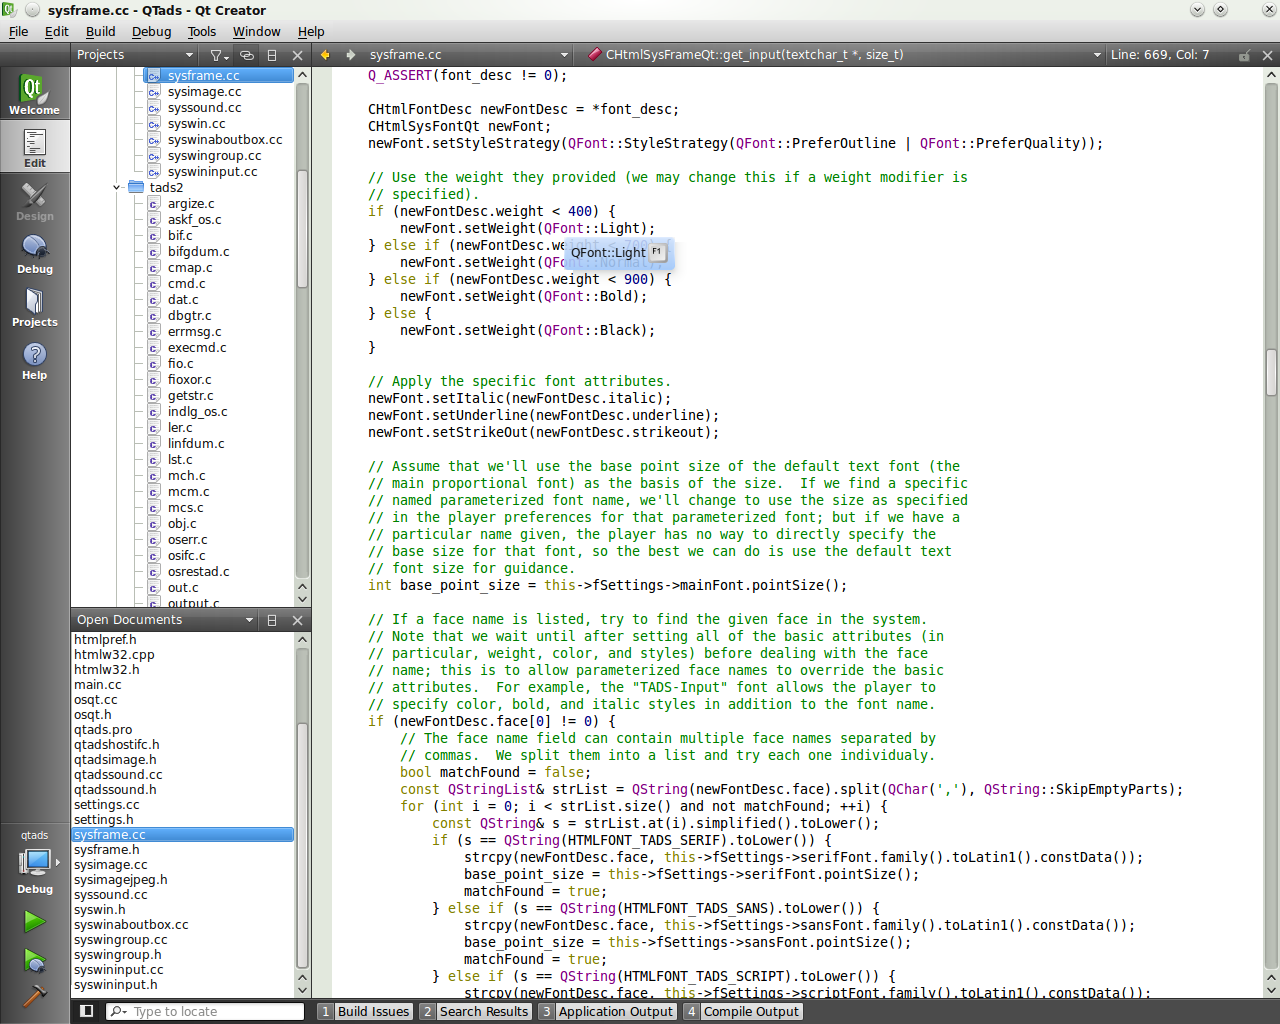
\includegraphics[width=0.8\textwidth]{img/general/QtCreator.png}
\caption{QtCreator Version 2.0.1 (Quelle: \protect\cite{qtcreator})}
\label{QtCreator}
\end{center}
\end{figure}

%Quellen:\\
%http://de.wikipedia.org/wiki/Qt_%28Bibliothek%29
%http://www.mathematik.uni-ulm.de/sai/ws02/cpp/070103/Qt.pdf
%http://wiki.ubuntuusers.de/Qt
%http://en.wikipedia.org/wiki/Qt_Creator


\section{Datenbank}
\label{section_Datenbank}

Um große Mengen an Daten effizient verarbeiten zu können, ist der Einsatz eines \ac{DBMS} ratsam (vgl. \citep{saake2010datenbanken}).

Für das Speichern von Daten und Betriebsparametern wird daher eine \ac{SQL} \ac{DB} benötigt. Bei der Wahl des \ac{DBMS}, stehen mehrere Systeme zur Auswahl. Dabei kommen SQLite und MySQL aufgrund der kostenlosen Verfügbarkeit in die engere Auswahl.
Beide System haben ihre Vor- und Nachteile.


\textbf{SQLite} ist ein \ac{SQL} \ac{DBMS}, welches ohne einen Server auskommt und operiert stattdessen in einer einzigen Datei. Alle Informationen wie Tabellenstruktur und Daten sind darin enthalten. Es wird vor allem im eingebetteten Bereich eingesetzt, da kaum Konfigurationen oder Verwaltung notwendig sind. Deshalb eignet es sich ausgezeichnet für sich schnell weiterentwickelnde Applikationen.
\\
Aufgrund dieser Eigenschaften existieren allerdings auch Nachteile. So unterstützt SQLite nur eingeschränkt mehrere Nutzer, die gleichzeitig auf die Datenbank zugreifen. Da das gesamte \ac{DBS} in einer einzigen Datei zusammengefasst ist, können mehrere zur selben Zeit durchgeführte Schreibzugriffe nicht unterstützt werden. Denn die einzige Zugriffskontrolle und Sicherstellung der Datenintegrität erfolgt durch das Dateisystem des Betriebssystem, was nicht immer fehlerfrei implementiert ist.
\\
Des Weiteren ist SQLite aufgrund des Ein-Datei-Systems nur eingeschränkt skalierbar. Bei einer größeren Datenmenge oder erhöhten Anzahl an Zugriffen ist es nicht möglich diese Datei auf mehrere Systeme zu separieren, um somit die Last gleichmäßig zu verteilen.

\textbf{MySQL} ist ein weiteres \ac{SQL} \ac{DBMS}, welches allerdings auf einer Serverarchitektur beruht. 
Es ermöglicht die Verwaltung von Nutzern und Rechten. Dadurch ist es ausgezeichnet für den gleichzeitigen Zugriff mehrerer Nutzer geeignet.\\ Außerdem ist das System gut hinsichtlich Performance und Größe zu skalieren, da die Last auf mehrere Server verteilbar ist. Zusätzlich bietet MySQL viele weitere Möglichkeiten für Performanceoptimierung, wie z.B. Query-Caching. Beim Query-Caching werden Ergebnisse von SQL-Abfragen (englisch: SQL-Query) zwischengespeichert, so dass sie bei erneuter Abfrage bereits vorliegen.
\\
Jedoch gibt es auch hier Nachteile. So ist die Konfiguration wesentlich schwerer und komplexer. Während bei SQLite kaum Konfigurationen nötig sind, müssen bei MySQL viele Einstellungen an das Host-System angepasst werden. Darunter fallen beispielsweise verschiedene Zwischenspeichergrößen und die Zugriffsrechte. Durch die Notwendigkeit eines Servers benötigt MySQL außerdem wesentlich mehr Ressourcen auf dem Host-System.

Für diese Arbeit eignet sich das relationale \ac{DBMS} MySQL besser. Auch wenn SQLite einige Vorteile im eingebetteten Bereich besitzt, ist die fehlende Unterstützen von mehreren Nutzern gleichzeitig ein Ausschlusskriterium.

\newpage

\section{Embedded Linux System}
\label{section_EmbeddedLinux}

Ein eingebettetes System (englisch: embedded system) ist laut  K. Bender (vgl. \cite{bender2005embedded}) ein Rechner, der in ein Gerät oder eine Maschine eingebettet ist und von außen nicht als solcher zu erkennen, sondern lediglich als Träger intelligenter Systemfunktionen sichtbar ist. Des Weiteren übernehme es dabei meist Überwachungs-, Steuerungs- oder Regelungsaufgaben.\\
Eingebettete Systeme sind oft spezifisch für die gegebene Aufgabe konzipiert. Dadurch ist es möglich die Hard- und Softwarekonfiguration des Systems zur Verminderung der Kosten und Maximierung der Leistung zu optimieren. Zu finden sind sie in den unterschiedlichsten Bereichen, beispielsweise in mobilen Geräten, industriellen Maschinen, Netzwerkhardware und Verbrauchergeräten.\ 

Ein Embedded Linux (deutsch: eingebettetes Linux) ist ein Betriebssystem, das auf dem Linux-Kernel basiert und in einem eingebetteten System zum Einsatz kommt. K. Yaghmour (vgl. \cite{yaghmour2008building}) sagt, dass Embedded Linux dabei typischerweise für ein Komplettsystem, bzw. ein Betriebssystem für ein spezifisches eingebettetes Gerät steht. Außerdem verwende man dabei den normalen Linux-Kernel, der sich lediglich in betriebsbedingten Eigenschaften des Zielsystems unterscheide.\ 

Das Embedded Linux System setzt sich aus einem Linux-Kernel nutzenden Rechner, dem Embedded Linux Betriebssystem mit für den Zielrechner passender Software und Werkzeugen für die Entwicklung zusammen. Diese Werkzeuge sind eine Entwicklungsumgebung mit Debugger und Cross-Compiler.

Der Vorteil bei der Verwendung des Linux Kernel ist u.a. die Abstraktion der Hardware. Über die Schnittstelle des Kernels kann mit einfachen Systemaufrufen mit der Hardware kommuniziert werden ohne die genaue Hardware zu kennen (siehe Abbildung \ref{figure_KernelHardwareLayer}).\\

\begin{figure}[h]
\begin{center}
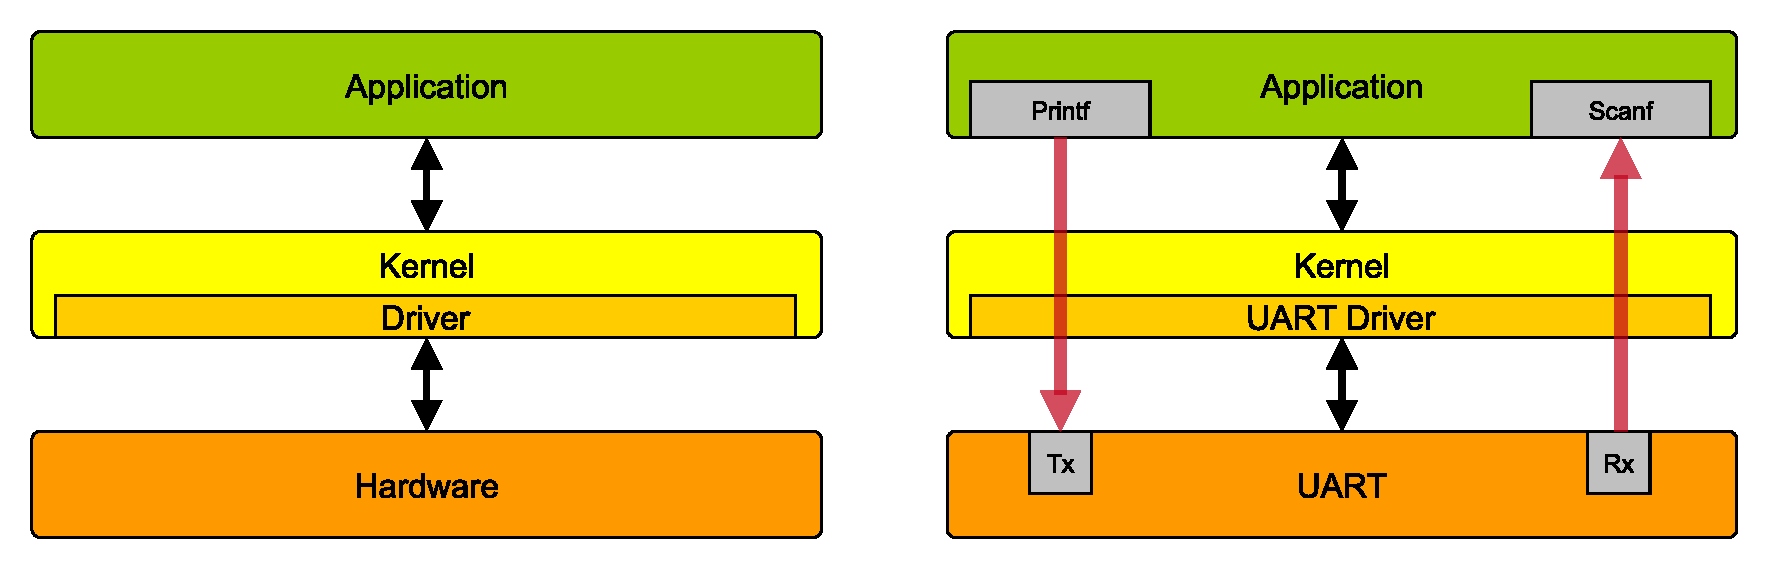
\includegraphics[width=\textwidth]{img/general/Kernel_Hardware_Layer.pdf}
\caption{Links:Kommunikation zwischen Applikation und Hardware.\\Rechts: Beispiel Kommunikation zwischen Applikation und UART über den Kernel.}
\label{figure_KernelHardwareLayer}
\end{center}
\end{figure}